\section{Empirical Evaluation}
\label{sec:evaluation}

\subsection{Experimental Setup}

\paragraph{Algorithms}

We implemented the low rank recovery optimization routines for $M_2$ and
$M_3$ using a proximal subgradient descent
algorithm.%\cite{candes11phaselift,tomioka2010estimation}. (Note sure about this citation and not required?)
The algorithm
was initialized with the regularized least squares solution and was run
for 500 iterations or until convergence up to a tolerance of $10^{-3}$. Both regularization parameters,
$\lambda_n^{(2)}$ and, $\lambda_n^{(3)}$ were annealed as $\frac{1}{n}$. 

As a baseline, we also implemented EM with two different
initializations. In the first, we used $\beta$s with random standard
Gaussian entries and uniform mixture probabilities, $\pi$. In the other,
we initialized EM with the starting points given by Spectral Experts. 

\paragraph{Datasets}

We generated synthetic data as follows:
First, we generated a vector $t$ sampled uniformly over the $b$-dimensional
unit hypercube $[-1,1]^b$.
Then, to get the actual covariates $x$, we applied a non-linear function of $t$
that conformed to the identifiability criteria discussed in
\sectionref{sec:algo}.
The coefficients $\{\beta_h\}$ were drawn from a standard Gaussian.  

As an example, one feature map we considered in the one-dimensional
setting was $x = (1, t, t^4, t^7)$. The data and the curves fit using
Spectral Experts, EM with random initializations and EM initialized with
the parameters recovered using Spectral Experts are shown in
\figureref{fig:curves}. We note that even on well-separated data such as
this, EM converged to the correct basin of attraction only 13\% of the time.

\begin{figure*}[p]
  \centering
  \subfigure[Spectral]{
    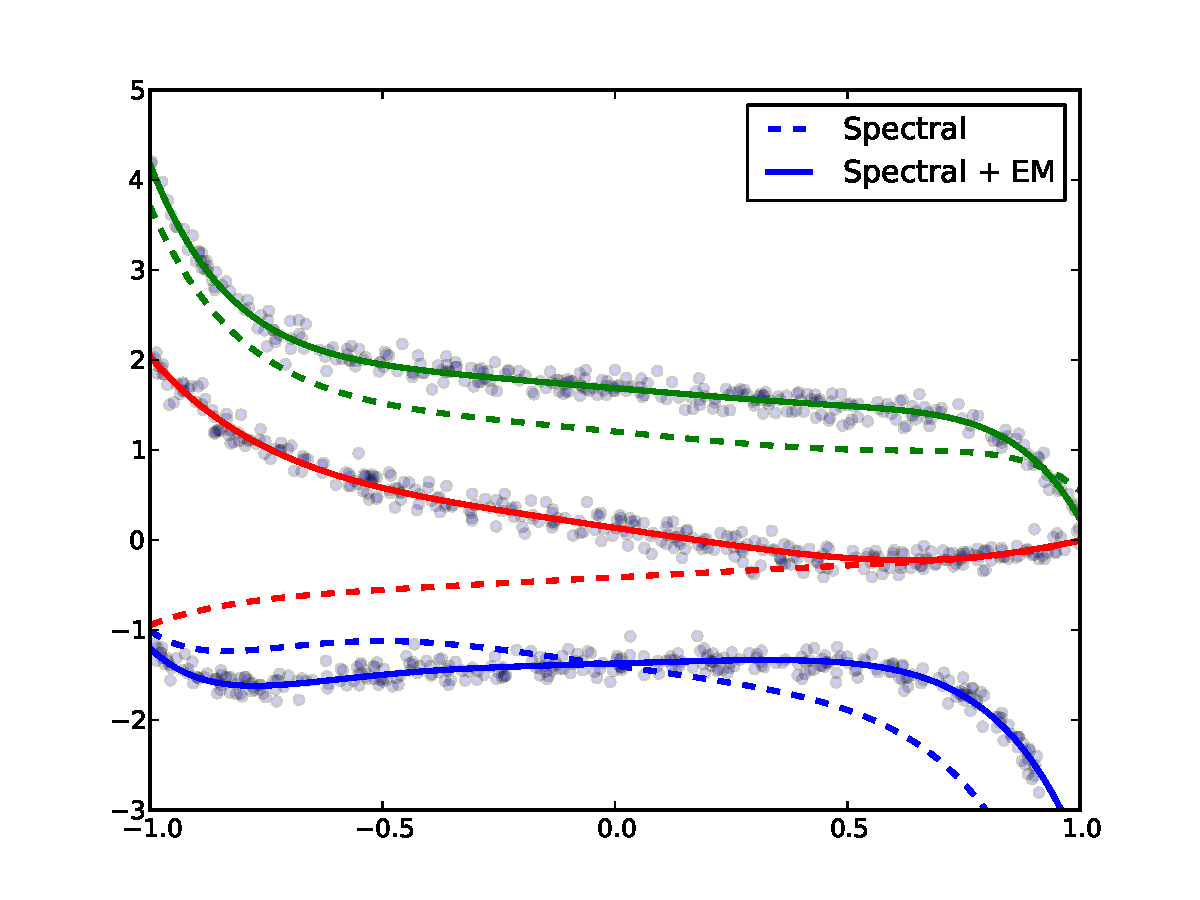
\includegraphics[width=0.50\textwidth]{figures/curves-vis/1-8-3-specm.pdf}}
    \hspace{-2em}
  \subfigure[EM]{
    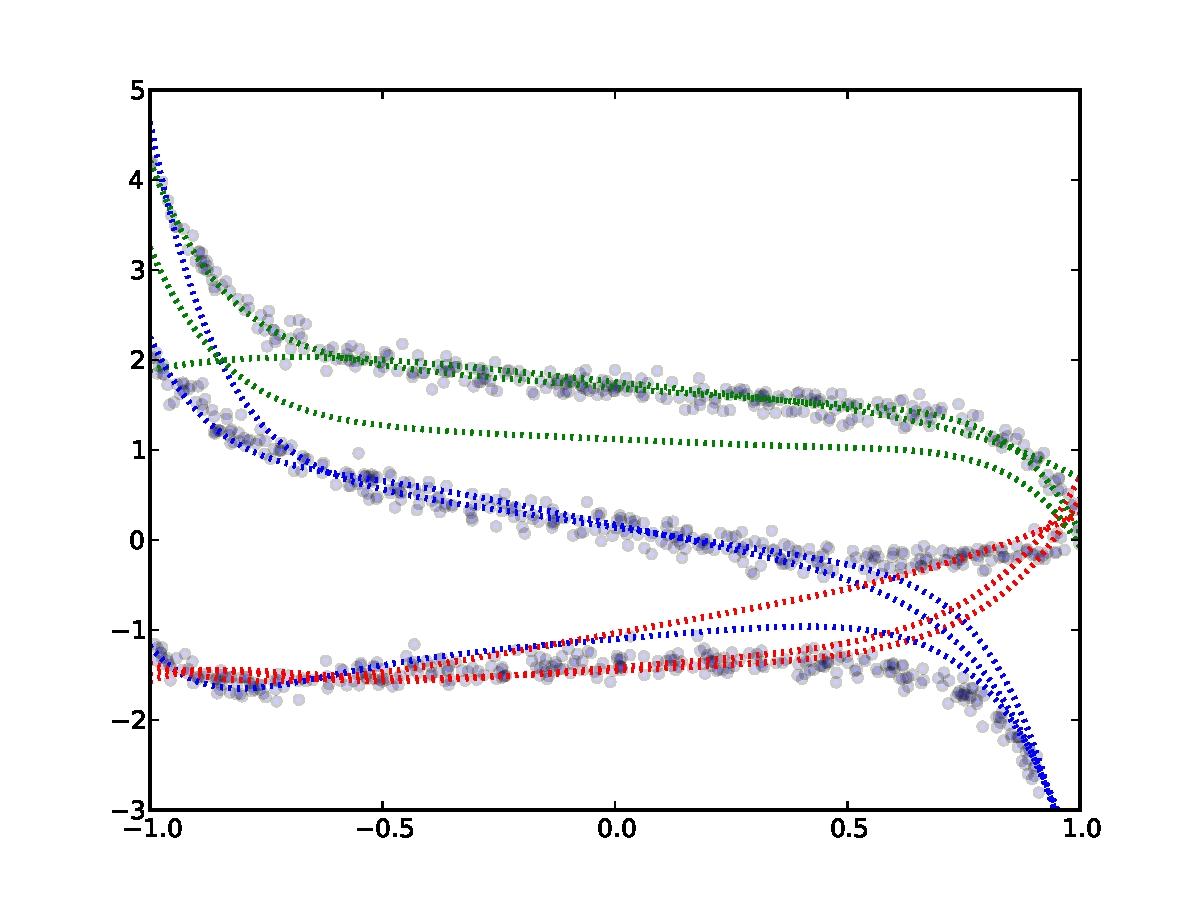
\includegraphics[width=0.50\textwidth]{figures/curves-vis/1-8-3-em.pdf}}
%  \subfigure[Spectral + EM]{
%    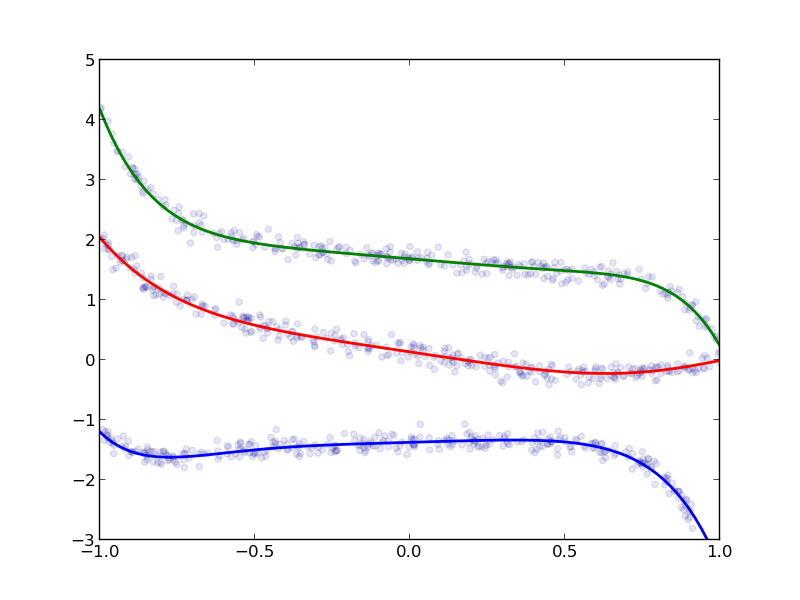
\includegraphics[width=0.34\textwidth]{figures/curves-vis/1-8-3-spem.png}}
  \caption{A comparison between Spectral Experts and EM. The dashed lines
  on the left denote the solution recovered by Spectral Experts. While
  not a perfect fit, it provides an good initialization for EM to find
  the true global minima. The dotted lines on the right show different
  local optima found by EM on this example.}
  \label{fig:curves}
\end{figure*}

%Default values:
%$n = 10^6$
%$k = 5$

\begin{table*}[p]
\caption{Parameter Recovery Error $\|\theta^* - \hat \theta\|_F$ ($N = 500,000$).}
\label{tbl:parameter-recovery}
\vskip 0.15in
\begin{center}
\begin{small}
\begin{sc}

  \begin{tabular}{ r r r c c c }
\hline
\abovespace\belowspace
Variables ($b$) & Features ($D$) & Components ($K$) & Spectral & EM & Spectral + EM \\
\hline
\abovespace
%$\{1$, $ x_1$, $ x_1^4\}$ 
  1 & 4 & 2 & 1.52 $\pm$ 0.71 & 0.28 $\pm$ 0.82 & {\bf 0.13 $\pm$ 0.55} \\
%$\{1$, $ x_1$, $ x_2$, $ x_1^2 x_2^2\}$ 
  2 & 5 & 2 & 2.92 $\pm$ 1.10 & 0.00 $\pm$ 0.00 & {\bf 0.00 $\pm$ 0.00} \\
  2 & 5 & 3 & 3.76 $\pm$ 1.93 & 0.43 $\pm$ 1.07 & {\bf 0.23 $\pm$ 0.76} \\
%$\{1$, $ x_1$, $ x_2$, $ x_1 x_2^3$, $ x_1^2 x_2^2$, $ x_1^3 x_2 \}$ 
  2 & 6 & 2 & 4.52 $\pm$ 1.67 & 0.63 $\pm$ 1.29 & {\bf 0.18 $\pm$ 0.66} \\
\belowspace
  2 & 6 & 5 & 6.78 $\pm$ 2.18 & 2.29 $\pm$ 1.79 & {\bf 1.77 $\pm$ 1.89} \\

%  2 & 5 & 3 & 1.87 $\pm$ 1.20 & {\bf 0.33 $\pm$ 0.96} & 0.35 $\pm$ 1.23 \\
% 2 & 6 & 5 & 5.27 $\pm$ 2.32 & 1.80 $\pm$ 1.80 & {\bf 1.51 $\pm$ 1.77} \\
%$\{1$, $ x_1$, $ x_2$, $ x_1 x_2^3$, $ x_1^2 x_2^2$, $ x_1^3 x_2$, $ x_1^3 x_2^4$, $ x_1^4 x_2^3 \}$ 
% 2 & 8 & 7 & 8.42 $\pm$ 1.66 & 7.41 $\pm$ 2.99 & {\bf 7.31 $\pm$ 2.47} \\
%$\{1$, $ x_1$, $ x_2$, $ x_3$, $ x_1 x_2 x_3^2$, $ x_1 x_2^2 x_3$, $ x_1^2 x_2 x_3$, $ x_1^2 x_2^2$, $ x_1^2 x_3^2$, $ x_2^2 x_3^2$, $ x_3^2\}$
% 3 & 10 & 3 & 3.78 $\pm$ 0.90 & 0.67 $\pm$ 1.49 & {\bf 0.51 $\pm$ 1.12} \\
%$\{1$, $ x_1$, $ x_2$, $ x_3$, $ x_1 x_2 x_3^2$, $ x_1 x_2^2 x_3$, $ x_1^2 x_2 x_3$, $ x_1^2 x_2^2$, $ x_1^2 x_3^2$, $ x_2^2 x_3^2$, $ x_3^2\}$
% 3 & 10  & 7 & 9.97 $\pm$ 3.22 & 1.43 $\pm$ 1.97 & {\bf 1.42 $\pm$ 2.17} \\

\hline

\end{tabular}
\end{sc}
\end{small}
\end{center}
\vskip -0.1in
\end{table*}

% \todo{Dataset 2: $b = 30$, $p = 1$. I'm unclear as to what we can show
% on this sort of data set. EM works extremely well, and the spectral
% methods do not converge easily.}

\subsection{Results}

\tableref{tbl:parameter-recovery} presents the Frobenius norm of the
difference between true and estimated parameters for the model, averaged
over 20 different random instances for each feature set and 10 attempts
for each instance. The experiments were run using $N = 500,000$ samples.

One of the main reasons for the high variance is the variation across
random instances; some are easy for EM to find the global minima and
others more difficult. In general, while the spectral algorithm did not
recover parameters extremely well, it provided a good initialization for
EM.

\begin{figure}[th]
  \centering
  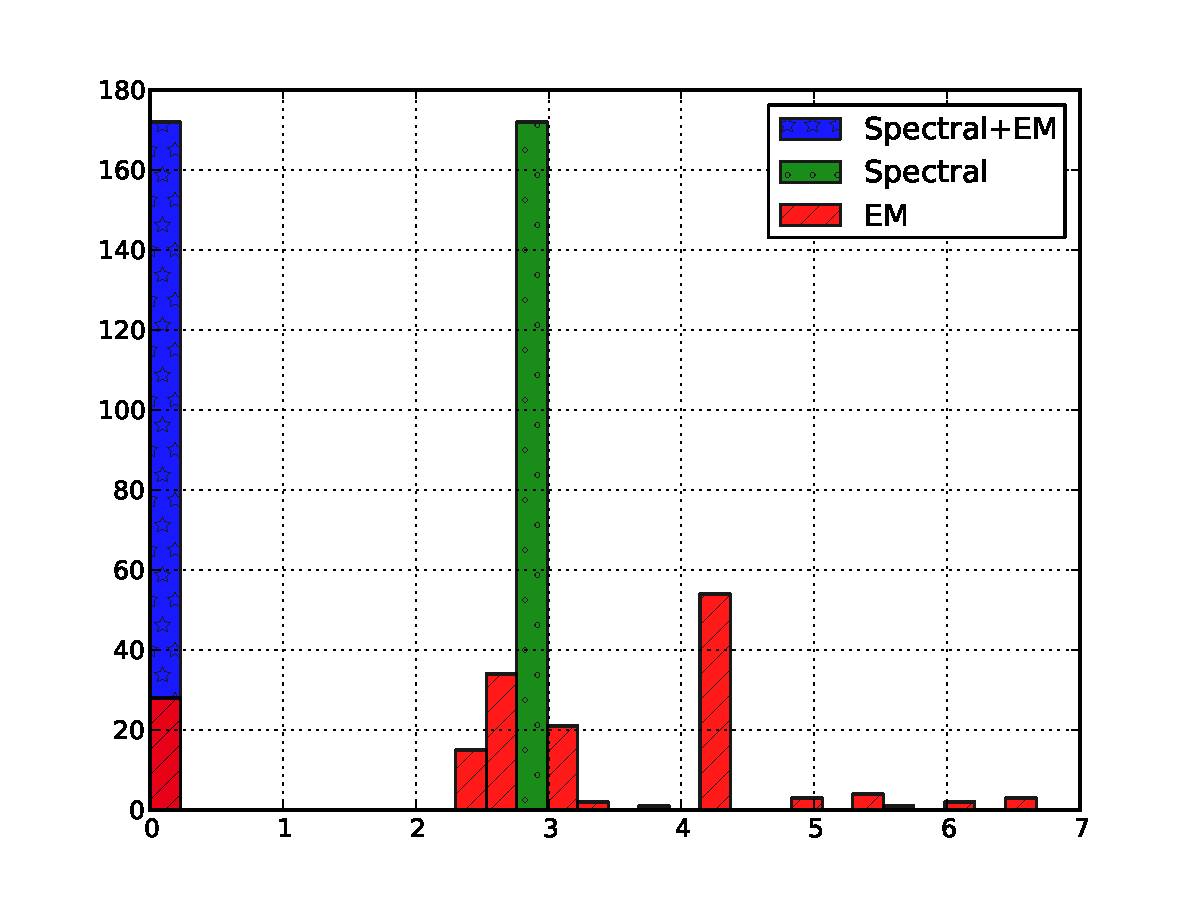
\includegraphics[width=0.50\textwidth]{figures/hist.pdf}
  \caption{Histogram over recovery errors between the three algorithms. $b = 1, d = 4, k = 3, N = 500,000$}
  \label{fig:hist}
\end{figure}

To study the stability of the solutions returned by the spectral method,
consider the histogram in \figureref{fig:hist}, which shows the recovery
errors of the algorithms over 170 attempts on a dataset with $b = 1, d = 4,
k = 3$. Typically, the spectral algorithm returned a stable solution.
When these parameters were close enough to the true parameters, we found
that EM almost always converged to the global optima. Randomly
initialized EM only finds the true parameters a little over 10\% of the
time and shows considerably higher variance. 

\paragraph{Effect of number of data points}

\begin{figure*}[p]
  \centering
  \subfigure[Well Data]{
    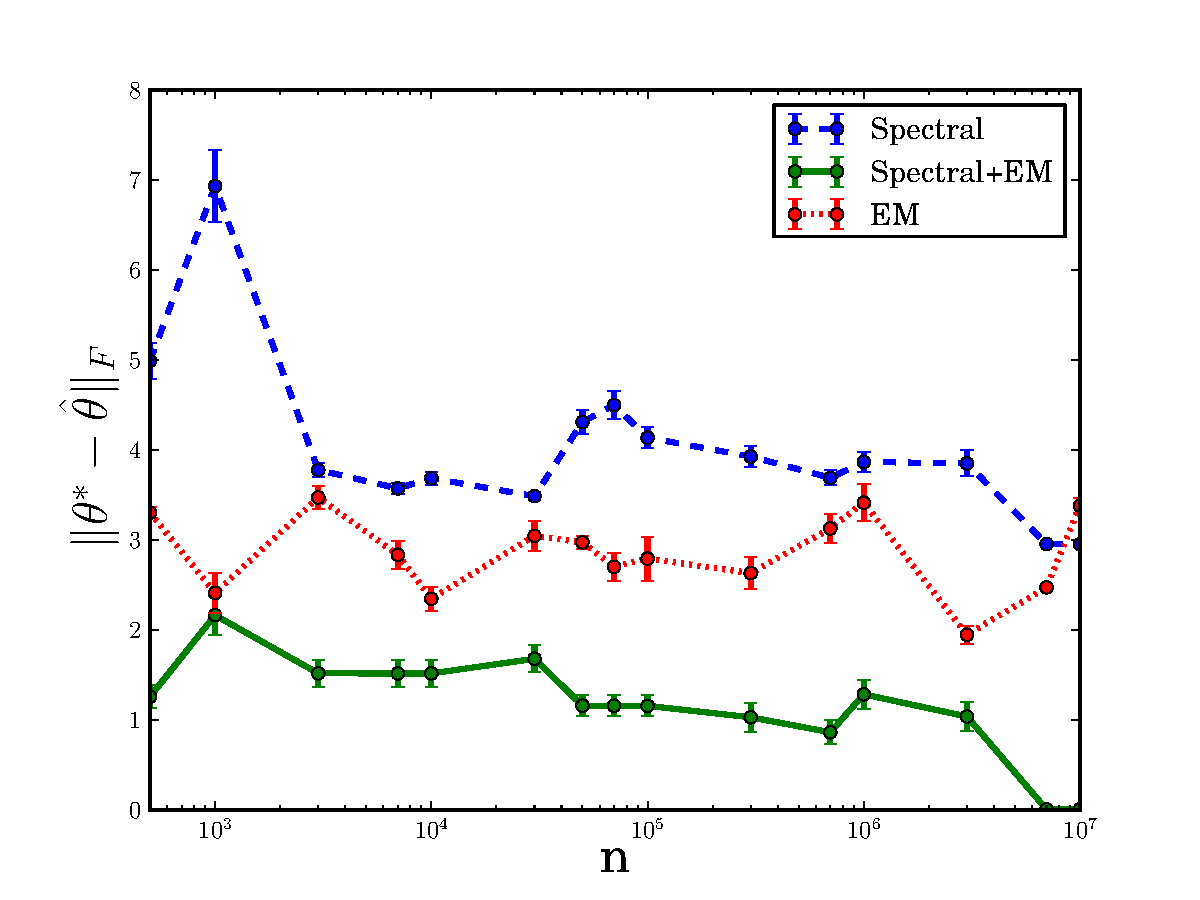
\includegraphics[width=0.50\textwidth]{figures/vs-n/1833-decay.pdf}
  }
    \hspace{-2em}
  \subfigure[Misspecified Data]{
    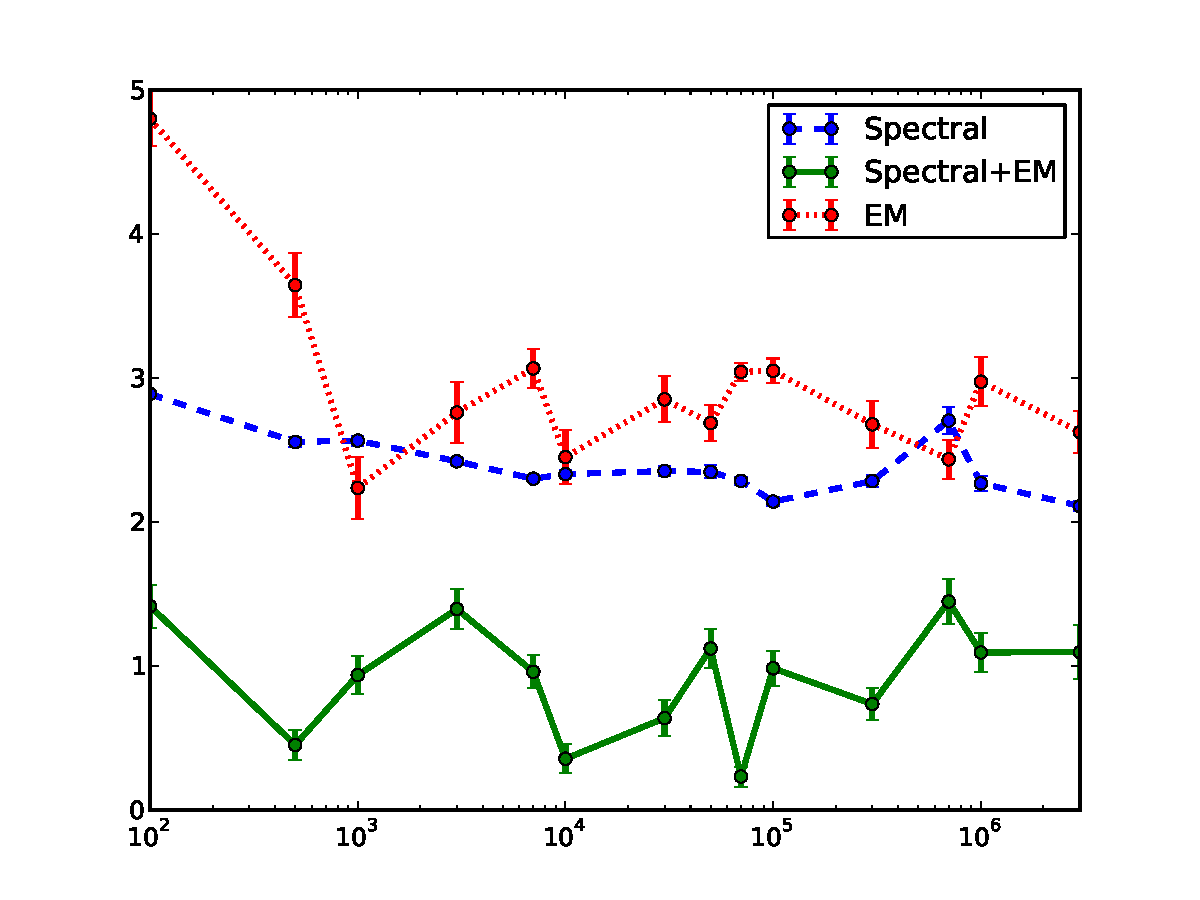
\includegraphics[width=0.50\textwidth]{figures/vs-n/1-8-3-3-rm.pdf}
  }
  \caption{Recovery error vs $n$  ($b = 1, d = 5, K = 3, N = 500,000$).}
  \label{fig:vs-n}
\end{figure*}

In \figureref{fig:vs-n}, we show how the recovery error varies as we get
more data. Each data point shows the mean error over 10 attempts, with
error bars. We note that the recovery performance of EM does not
particularly improve; this suggests that EM continues to get stuck in
a local optima. The spectral algorithm's error decays slowly, and as it
gets closer to zero, EM initialized at the spectral parameters finds the
true parameters more often as well. This behavior highlights the
trade-off between statistical and computational error. 

\paragraph{Misspecified Data}

\begin{table*}[t]
\caption{Parameter Recovery Error $\|\theta^* - \hat \theta\|_F$ with misspecified data ($N = 500,000$).}
\label{tbl:parameter-recovery-mis}
\vskip 0.15in
\begin{center}
\begin{small}
\begin{sc}

  \begin{tabular}{ r r r c c c }
\hline
\abovespace\belowspace
Variables ($b$) & Features ($d$) & Components ($K$) & Spectral & EM & Spectral + EM \\
\hline
\abovespace
 1 & 4 & 2 &  2.94 $\pm$ 1.52 & 0.29 $\pm$ 0.85 &  {\bf 0.22 $\pm$ 0.72} \\
\belowspace
 2 & 5 & 3 &  3.82 $\pm$ 2.00 & 0.44 $\pm$ 1.12 &  {\bf 0.35 $\pm$ 1.00} \\
 2 & 6 & 5 &  9.89 $\pm$ 4.46 & {\bf 2.53 $\pm$ 1.77} &  2.69 $\pm$ 1.83 \\
 2 & 8 & 7 & 23.07 $\pm$ 7.10 & 9.62 $\pm$ 1.03 &  {\bf 8.16 $\pm$ 2.31}  \\
\hline

\end{tabular}
\end{sc}
\end{small}
\end{center}
\vskip -0.1in
\end{table*}

To evaluate how robust the algorithm was to model mis-specification, we
removed large contiguous sections from $x \in [-0.5,-0.25] \cup
[0.25,0.5]$ and ran the algorithms again.
\tableref{tbl:parameter-recovery-mis} reports recovery errors in this
scenario. The error in the estimates grows larger for higher $d$.

